\chapter{RCNSP的设计与实现}
本章介绍规则自动补全的神经符号VQA框架(Rule Complement Neuro-Symbolic Pipeline, RCNSP),
下面分别从RCNSP设计方案、RCNSP核心技术及实现、实验分析三个方面进行详细阐述。
\section{RCNSP设计方案}
RCNSP框架的架构设计方案如图\ref{fig:pipeline}所示。框架的整体设计思路是:
在框架初始化阶段,规则蒸馏模块依据LLM中蕴含的大量知识生成ASP规则,进而获得较为完整的ASP知识库。
在框架运行阶段,视觉场景理解模块从输入的图像中抽取
物体所在区域、物体属性等信息,并以ASP形式进行表示;另一方面,语义解析模块对输入的自然语言问题进行解析,
同样以ASP形式进行表示,并由规则修正模块对生成的ASP规则进行修正。
随后将ASP知识库、图像、问题三个方面的ASP规则统一输入ASP推理模块进行求解。如果对某个问题无法求解出正确答案,
规则蒸馏模块会尝试进行生成新规则,实现ASP知识库的动态更新。
最后,由于ASP推理模块输出的是ASP语句,
可读性较差,普通用户难以理解,因此需要求解结果翻译模块将其翻译为自然语言形式进行输出。
\begin{figure}[h]
    \centering
    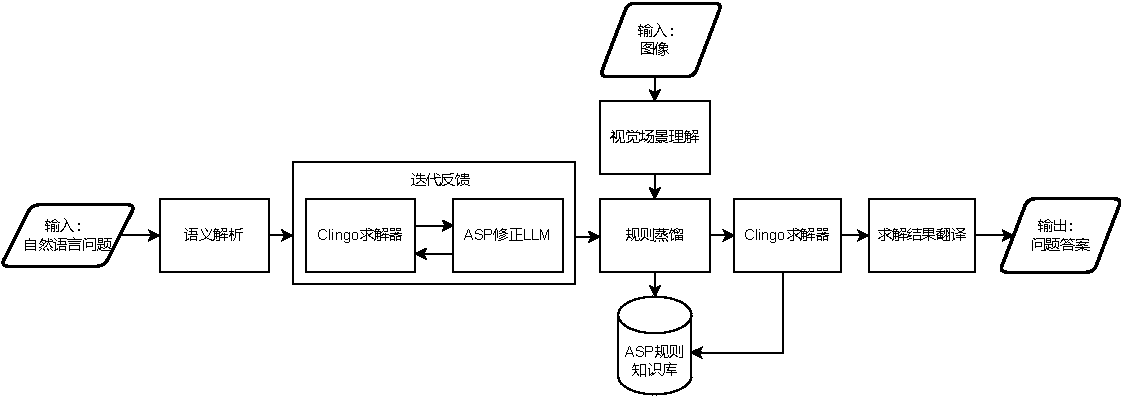
\includegraphics[width=\textwidth]{figures/pipeline-crop.pdf}
    \caption{面向空间推理领域的神经符号框架示意图}
    \label{fig:pipeline}
\end{figure}
\subsection{视觉场景理解}
本模块的任务是从输入的积木世界图像中检测积木物体并提取其属性(颜色、形状、大小、材质)、位置以及相互之间的空间关系,并把
这些视觉信息转换为符号化的ASP事实(如\texttt{color(obj1,red)}、\texttt{shape(obj1, cube)}、\texttt{left(obj1,obj2)}等)。

本模块在研究中面临的挑战主要有:在部分积木世界图像中,可能会出现物体密集或者遮挡严重的复杂场景,GLIP可能会出现目标区域重叠导致的多重检测
或者误检问题,进而影响后续语义解析与推理模块的准确性。

技术方法上,本文使用GLIP作为目标检测模型,GLIP完成目标检测后,经空间位置提取、空间关系提取后,生成该图像对应使用ASP表示的场景。
同时,采用非极大值抑制以及深度信息辅助过滤的方法,来解决目标检测中遇到的难点。

现有的神经符号VQA框架不支持图像输入,不能完成积木世界VQA任务,本文引入视觉场景理解模块,使RCNSP具备现有神经符号VQA框架所不支持
的处理多模态输入的能力。
\subsection{语义解析}
语义解析模块的目标是将用户的自然语言问题转化为能够准确反映积木世界VQA问题且语法和语义均正确的ASP查询,以支持后续推理。
本模块的研究中的难点在于,如何在训练LLM生成ASP程序的相关数据集较少的情况下,指导LLM准确生成ASP程序。

技术方法上,本模块采用提示词优化的方法对LLMs进行优化,并引入DSPy作为提示管理的框架,
针对POVQAD中积木世界VQA的4类属性查询问题设计了共28种提示词以训练LLMs准确生成对应的ASP程序,此外设计了
同时考察语法正确和语义正确两方面的自定义评价函数\texttt{ValidScore},用以指导DSPy的 FewShotPromptOptimizer 优化器对提示词进行优化。

相较于通用的LLMs生成ASP程序的方法,本模块的方法更专注于POVQAD中4类问题的语言特性,
能够更准确高效地处理涉及物体属性和空间关系的问题,减少歧义解析的错误率。
\subsection{规则修正}
本模块的任务是在通过语义解析模块得到ASP查询之后,进行多轮迭代检查与修正,确保ASP查询正确无误,可以顺利通过Clingo执行。
本模块研究中的难点在于,LLM在生成ASP规则时容易出错,且目前学术界和工业界很少有针对积木世界VQA相关的ASP程序进行修正的微调数据集,
难以采用微调的方法对生成ASP规则进行优化。

技术方法上,本文设计了多种提示模板,通过DSPy框架对LLM进行提示词优化,使模型在无需重新训练的情况下,自动学习如何更有效地修正 ASP 程序,
同时提示词优化降低了对大量高质量标注数据的需求,很大程度上解决了本模块研究中的难题。

本方法相比已有工作的创新点在于,已有工作中的ASP代码修正依赖于预先定义的ASP错误类型和修正策略。而本方法通过引入Clingo的执行反馈提示,
指导提示词的动态变化,在保持模型参数不变的前提下,显著提高了ASP程序的可执行性和准确率。
\subsection{规则蒸馏}
本模块旨在从LLMs中提取简洁且准确的ASP规则,用于积木世界的推理任务。
具体应用主要包括两方面:一是在RCNSP初始化阶段,利用“LLMs基于海量语料预训练,包含
丰富的知识”这一特性,将LLMs中蕴含的知识转换为可执行、可解释的ASP规则的,用于完善初始ASP知识库。
二是在RCNSP运行阶段,当出现对某个问题无法求解出正确答案的情况时,
规则蒸馏模块会尝试进行生成新规则,实现ASP知识库的动态更新。

本模块研究的难点在于,在RCNSP初始化阶段对积木世界VQA数据集进行蒸馏的过程中,当样本的数量过多时,进行全量蒸馏
可能会耗时过长,同时也能会引入一些对解决积木世界VQA问题无关的冗余知识。这些冗余知识在每次ASP推理时,都要输入到Clingo中,
当RCNSP处理用户VQA请求数量逐步增加时,因冗余知识而导致的累计性能损耗也将逐步增大。

技术方法上,本模块通过构建初始ASP知识库,并以本文构建的积木世界数据集POVQA\-D为样本进行蒸馏,生成积木世界空间推理所需的ASP规则并完善ASP知识库。
另外在RCNSP运行过程中,当出现知识不足,无法求解的情况时,规则蒸馏模块将会引导LLM生成新的ASP规则以补充ASP知识库。
同时,本模块在蒸馏过程中采用了样例选择策略,减少无关数据的干扰,避免全量蒸馏,实现了蒸馏性能优化,解决了本模块研究中的难点。

与已有工作中传统的模型压缩式蒸馏不同,本方法强调将LLM中“隐式的知识”显式地提取为ASP规则。
而规则蒸馏的本质是将大语言模型中蕴含的知识,转换为可执行、可解释的逻辑规则,用于扩展已有的推理系统。
\begin{enumerate}[nosep]
\item \textbf{启发式拓展}:以经迭代反馈修正后得到的ASP规则和视觉场景理解模块生成的ASP规则为基础,当发现这些ASP规则无法解答某个问题时,引导LLM生成新的规则。
\item \textbf{以数据为指导而非训练为导向}:不训练模型,而是以示例为提示,向LLM提出规则生成任务。
\end{enumerate}
\subsection{ASP推理}
ASP推理模块的功能是:根据输入图像的ASP表示、ASP知识库中的ASP规则、经过修正后自然语言问题对应的ASP查询,
共同输入到Clingo,生成答案集。

\subsection{求解结果翻译}
求解结果翻译模块的功能是:将ASP推理模块输出的答案集,经LLM处理将其转换为自然语言形式的答案。
\section{RCNSP核心技术及实现}
\subsection{视觉场景理解}
本节主要围绕视觉场景理解的流程展开详细阐述,具体包括目标检测、空间位置提取、空间关系提取以及场景生成这四个环节。
最后,给出一个完整的视觉场景理解演示案例,并讨论在实现过程中遇到的关键技术挑战及相应解决方案。
\subsubsection{目标检测}
本文采用了GLIP模型作为目标检测的核心工具,其主要优势体现在:
\begin{enumerate}[nosep] 
\item \textbf{语言-视觉预训练能力:}GLIP在大规模图文对数据上进行预训练,能够根据自然语言描述(例如“红色立方体”)直接定位图像中的对应物体,从而实现图像内容与问题描述的高效对齐; 
\item \textbf{高效性与鲁棒性:}模型在处理多样化场景时具有较高的检测准确率,适合构造后续依赖视觉信息的场景图。 
\end{enumerate}

具体实现流程如下:
\begin{enumerate}[nosep] 
\item \textbf{图像预处理:}将原始图像调整至GLIP模型要求的输入分辨率(例如800$\times$1333像素),
以保证检测精度; 
\item \textbf{文本提示构造:}根据POVQAD数据集,设计一组覆盖目标类别及属性的自然语言提示。
本文选取的提示短语包括描述物体大小(如“大物体”、“小物体”)以及颜色与形状组合(如“红色立方体”、“蓝色球体”、“绿色圆柱体”等); 
\item \textbf{目标检测与属性解析:}将图像和文本提示输入GLIP,获得每个检测物体的边界框和类别标签。随后对类别标签进行解析,将复合描述(如“红色立方体”)拆解为单独属性(color=red, shape=cube)。同时,通过计算边界框面积($(x_2 - x_1)\times(y_2 - y_1)$),结合预设阈值进一步推断物体的大小属性。 
\end{enumerate}

例如,对于一张包含“红色立方体”和“蓝色球体”的图像,GLIP可能检测出如下信息: 
\begin{enumerate}[nosep] 
\item 物体1:类别为“红色立方体”,边界框坐标为$(x_1, y_1, x_2, y_2)$; 
\item 物体2:类别为“蓝色球体”,边界框坐标为$(x_3, y_3, x_4, y_4)$。 
\end{enumerate}
\subsubsection{空间位置提取}
在完成目标检测后,接下来的任务是为每个物体确定其精确的空间位置,这对于后续空间关系的推理至关重要。
本文采用以下两种方式提取物体位置信息:
\begin{enumerate}
\item \textbf{二维中心点计算}:利用目标检测得到的边界框信息,计算物体在图像平面内的中心点坐标。公式如下:
$$x_c = \frac{x_1+x_2}{2}, y_c = \frac{y_1 + y_2}{2}$$
该中心点坐标用于描述物体在二维图像中的位置;
\item \textbf{三维位置信息获取}:若图像同时包含深度信息(例如通过Blender渲染生成的场景),则可直接从深度图中提取物体的z值,从而获得物体在三维空间中的位置,
表示为$(x, y, z)$。
\end{enumerate}

提取出的位置信息将以ASP事实的形式进行存储,例如:position(obj1, x1c, y1c, z1) 表示物体1的中心点位置。
\subsubsection{空间关系提取}
空间关系的提取是实现复杂场景理解与多步逻辑推理的关键。本文从以下几个角度对空间关系进行提取:
\begin{enumerate}[itemsep=0.5em] 
\item \textbf{二维空间关系:}基于物体的中心点坐标计算物体之间的相对位置。例如: 
    \begin{itemize}[leftmargin=2em] 
        \item 若物体A的$x_c$小于物体B的$x_c$,则判定A位于B的左侧,表示为\texttt{left(objA, objB)}; 
        \item 类似地,通过比较$y_c$坐标可判定上下关系(例如,若物体A的$y_c$小于B,则A在B之上,记作\texttt{above(objA, objB)})。 
    \end{itemize} 
\item \textbf{三维空间关系:}利用深度信息,对物体间的前后关系进行判断。
例如,若物体A的z值小于物体B的z值,则判定A位于B的前面,记作\texttt{in\_front\_of(objA, objB)}。 
\item \textbf{遮挡关系:}结合边界框重叠情况与深度信息进行判断。如果两个物体边界框存在重叠且A的深度值明显小于B,
则可以认为A遮挡B,记作\texttt{occludes(objA, objB)}。 
\end{enumerate}
所有提取到的空间关系均转换为ASP事实,如:
left(obj1, obj2) 表示物体1在物体2的左边,in\_front\_of(obj1, obj2) 表示物体1在物体2的前面;
occludes(obj1, obj2) 表示物体1遮挡了物体2。
\subsubsection{场景图生成}
场景图是将目标检测、空间位置与空间关系综合融合成的统一结构化表示,使用ASP作为表示形式,其主要构成如下: 
\begin{enumerate}[nosep] 
    \item \textbf{节点表示:}每个节点对应图像中的一个物体,并附有相应的属性(如color, shape, size, material)以及位置信息; 
    \item \textbf{边的构建:}节点之间的边用于表示物体间的空间关系,如left\_of、in\_front\_of等。 
\end{enumerate}

在构建过程中,首先为每个检测到的物体创建一个节点,并记录其属性及位置;
随后,依据前述空间关系,将相应的有向边添加到图中。
最终,整个场景图将被转化为ASP事实,以支持后续符号推理任务。
\subsubsection{实现细节与实例}
为便于说明,下面给出一个具体示例。假设输入图像包含如下场景: 
\begin{enumerate}[nosep] 
    \item 一个红色大立方体位于图像左侧; 
    \item 一个蓝色小球体位于图像右侧,且位于红色立方体的前方。 
\end{enumerate}

经过GLIP目标检测,得到如下检测结果: 
\begin{itemize}[itemsep=0pt,parsep=0pt] 
    \item 物体1:类别为“红色立方体”,边界框为(50, 100, 150, 200); 
    \item 物体2:类别为“蓝色球体”,边界框为(250, 50, 350, 150)。 
\end{itemize}

进一步计算得到: 
\begin{itemize}[itemsep=0pt,parsep=0pt] 
    \item 物体1的中心点坐标为$(100,150)$; 
    \item 物体2的中心点坐标为$(300,100)$。 
\end{itemize}

假设深度信息显示:物体1的z值为50,物体2的z值为75,则可提取以下空间关系: 
\begin{itemize}[itemsep=0pt,parsep=0pt] 
    \item \texttt{left\_of(obj1, obj2)}(因为100 $<$ 300); 
    \item \texttt{above(obj2, obj1)}(因为100 $<$ 150); 
    \item \texttt{in\_front\_of(obj2, obj1)}(因为75 $>$ 50,在三维空间中深度值较大的物体更靠后,需根据具体定义调整)。 
\end{itemize}

最终生成的ASP事实示例如下: 
\begin{lstlisting}[language=Prolog] 
color(obj1, red). 
shape(obj1, cube). 
size(obj1, large). 
position(obj1, 100, 150, 50).

color(obj2, blue). 
shape(obj2, sphere). 
size(obj2, small). 
position(obj2, 300, 100, 75).

left(obj1, obj2). 
above(obj2, obj1). 
in_front_of(obj2, obj1). 
\end{lstlisting}
\subsubsection{技术挑战与解决方案}
在处理物体密集或遮挡严重的复杂场景时,GLIP 可能会出现目标区域重叠导致的多重检测或误检问题,
进而影响后续语义解析与推理模块的准确性。主要表现为:当多个物体近距离排列或相互遮挡时,模型可能无法准确区分边界,
导致同一物体被多次检测或部分遮挡物体被误识别为其他类别。

为了解决上述问题,本文引入两种策略对 GLIP 的检测结果进行后处理优化:非极大值抑制(Non-Maximum Suppression, NMS)
和深度信息辅助过滤(depth-assisted filtering),以提高目标检测的精度与鲁棒性。

非极大值抑制是一种经典的候选框去重技术,其基本思想是:在多个候选框预测同一目标时,保留置信度最高的框,
并删除与之重叠度(IoU)较高的其他框。在本文中,我们针对GLIP输出的所有检测框,按照类别相关的置信度进行排序,
并设置IoU阈值(如0.5),执行NMS操作。这一策略可以显著减少对同一目标的重复检测现象,从而降低伪阳性率,尤其在密集物体场景中成效明显。

虽然NMS能有效处理重叠问题,但在遮挡严重的场景中,单纯依赖二维图像信息可能仍存在遮挡物体错误识别为其他类别的风险。
为此,本文进一步引入场景的深度图信息作为辅助特征,用于分析候选目标的深度一致性。
在具体实现中,我们利用深度图对检测框区域内的深度值进行统计,对深度波动异常大或与周围区域差异显著的框进行剔除或降权处理。
该方法能够有效识别被遮挡或边缘模糊的虚假目标,提高复杂场景下检测的精度。
\subsection{语义解析}
为了让LLM更准确地生成积木世界VQA任务中的ASP程序,本文在此对通用LLM进行提示词优化,
并且引入DSPy作为提示管理与语义生成框架,以构建结构化、模块化、可优化的语义解析流程。
本节按照任务定义、提示词设计、提示词优化、输出的顺序进行介绍。
\subsubsection{任务定义}
DSPy是一个面向语言任务的程序性提示框架,能够在具备结构化的输入输出约束的前提下,
调用LLM完成特定子任务。在语义解析模块中,将“问题$\rightarrow$ASP程序”建模为一个标准的DSPy模块,
定义其输入为英文问题,输出为符合ASP语法的逻辑规则字符串。

在实现上,通过DSPy的\texttt{Signature}定义任务结构,其中明确了模块的目标,即
根据输入问句生成问题所对应的ASP逻辑表示。
\begin{lstlisting}
class ParseQuestionToASP(Signature):
    question = dspy.InputField(desc="问题")
    asp_code = dspy.OutputField(desc="ASP程序片段")
\end{lstlisting}
\subsubsection{提示词设计}
本文对第三章中构建的积木世界VQA数据集POVQAD的问题进行分析,对4种问题(分别提问物体的颜色、形状、大小、材质)分别设计提示词。
考虑到POVQAD中问题表述的多样性,每种问题的提示模板均有多种形式。以下对4种问题分别展示一种提示词。所有提示词(共计28种)
在附录\ref{appendix:semantics-parsing-prompts}中予以展示。
\begin{enumerate}[nosep]
\item \textbf{颜色查询}:问题对物体的颜色属性进行提问,本文共为颜色类问题设计了7种提示模板,以下是一个示例。
\begin{lstlisting}
任务描述:你是一个AI助手,负责将英文问题转换成ASP逻辑语言。
问题:What is the color of the cylinder to the right of the blue sphere?
ASP程序:
missing(Q):-has_property(X,color,Q),has_property(X,shape,cylinder),
    has_property(X1,color,blue),has_property(X1,shape,sphere),
    right(X1,X).
\end{lstlisting}
\item \textbf{形状查询}:问题对物体的形状属性进行提问,本文共为颜色类问题设计了7种提示模板,以下是一个示例。
\begin{lstlisting}
任务描述:你是一个AI助手,负责将英文问题转换成ASP逻辑语言。
问题:What shape is the blue object left of the medium blue rubber object on the right side of the big object right of the small cyan rubber cone ?
ASP程序:
missing(Q):-has_property(X,shape,Q),has_property(Y3,shape,cone),
    has_property(X,color,blue),has_property(Y1,color,blue),
    has_property(Y1,size,medium),has_property(Y3,size,small),
    has_property(Y3,material,rubber),has_property(Y2,size,large),
    has_property(Y3,color,cyan),has_property(Y1,material,rubber),
    left(Y1,X),right(Y2,Y1),right(Y3,Y2),
    X!=Y1,Y1!=Y2,Y2!=Y3,X!=Y2,X!=Y3,Y1!=Y3.
\end{lstlisting}
\item \textbf{大小查询}:问题对物体的大小属性进行提问,本文共为颜色类问题设计了6种提示模板,以下是一个示例。
\begin{lstlisting}
任务描述:你是一个AI助手,负责将英文问题转换成ASP逻辑语言。
问题:There is another gray object that is made of the same material as the cyan cone ; what is its size ? 
ASP程序:
missing(Q):-has_property(X,size,Q),X!=Y,has_property(Y,color,cyan),
    has_property(Y,shape,cone),has_property(X,color,gray),
    same_material(Y,X).
\end{lstlisting}
\item \textbf{材质查询}:问题对物体的材质属性进行提问,本文共为颜色类问题设计了8种提示模板,以下是一个示例。
\begin{lstlisting}
任务描述:你是一个AI助手,负责将英文问题转换成ASP逻辑语言。
问题:What is the material of the other red thing that is the same shape as the big thing ? 
ASP程序:
missing(Q):-has_property(X,material,Q),X!=Y,has_property(Y,size,large),
    has_property(X,color,red),same_shape(Y,X).
\end{lstlisting}
\end{enumerate}

最终在\texttt{PromptModule}中设定统一提示模板,引导模型按照所示结构生成ASP程序。
\subsubsection{提示词优化}
为进一步提升提示效果,本文引入验证集驱动的提示优化策略。本文随机选取POVQAD中部分问题及对应ASP表示,组成验证集,通过
语法准确率和语义准确率,对few-shot示例顺序与提示模板进行自动调整。

此处采用DSPy提供的 FewShotPromptOptimizer 优化器,以ASP程序的语法正确率和语义正确率作为评价指标,训练优化提示内容:
\begin{lstlisting}
optimizer = FewShotPromptOptimizer(devset=dev_questions, metric=asp_valid_score)
optimized_parse_module = optimizer(parse_module)
\end{lstlisting}

DSPy提供了FewShotPromptOptimizer、ReActPromptOptimizer、ChainOfThoughtOptimizer等多种提示词优化器,本文在此处选用
FewShotPromptOptimizer主要基于以下几点考量:
\begin{enumerate}[nosep]
\item 积木世界VQA的语义解析任务,也即根据自然语言问题生成其对应的ASP查询程序,本质上“结构化映射”而非“多轮推理”,属于结构预测任务。
并不需要模型生成复杂的思维链条或搜索多个中间步骤,因此并不适合使用 ReActPromptOptimizer 或 ChainOfThoughtOptimizer 这类用于逐步思考与规划的优化器。
\item 在任务定义中,已经确定了清晰的输入输出结构,并且已经根据POVQAD中4类问题的特点构造了28个“问题-ASP程序”示例对。
FewShotPromptOptimizer 正是专门用于自动选择、排列、剪枝、重组这些示例对以提升提示效果的优化器,它能用验证集度量“哪组few-shot示例组合效果最好”,无需引入额外监督。
\item FewShotPromptOptimizer完全不依赖 LLM 微调,也不需要多轮推理轨迹采集,训练稳定、开销小,适合结构化语言映射任务。
此外,相比 ReActPromptOptimizer,它不需要考虑中间推理路径,因此构造门槛更低。
\item FewShotPromptOptimizer 的核心机制是“提供格式完好的示例”,它能有效帮助LLM学到一致的生成模式,
而 ReActPromptOptimizer 或 ChainOfThoughtOptimizer 更强调思维路径,反而容易引入不必要的多样性或碎片化表达,进而
可能导致输出的ASP程序在格式、句法上出现错误。
\end{enumerate}

上述优化器中的参数\texttt{asp\_valid\_score}为自定义评价函数,用于判断LLM输出的ASP程序是否满足语法正确和语义正确。下面对如何定义并计算自定义评价
函数的值给出相关解释:

对于一个程序$P$,Clingo用于计算该程序的答案集。
进而该过程可以等价于:定义一个函数$f(P) = AS(P)$,其中$AS(P)$表示程序P的所有回答集(可能为空)。
LLM根据提示$x$生成的ASP程序,记为$y ~ P_L(|x)$。与$x$对应的能够真实表示问题的标准ASP程序,记为$y^*$。按照以下步骤来进行验证:
首先基于$x$构建一个表示具体实例的事实集$F_{y^*}$。接着,构造两个完整的ASP程序:
\begin{enumerate}[nosep]
\item $P = y \cup F_{y^*}$:由模型生成程序与事实集合成的程序。
\item $P^* = y^* \cup F_{y^*}$:由标准程序与事实集合成的程序。
\end{enumerate}

此后,执行以下评估步骤:
\begin{enumerate}[nosep]
\item 语法检查。该步骤的执行结果记作$syntax$。调用Clingo运行程序$P$,若未发生解析错误,则认为模型生成的程序 $y$ 在语法上是正确的,则判定为语法命中,记$syntax = 1$。否则,则判定为不命中,记$syntax = 0$。
\item 语义检查。该步骤的执行结果记作$semantic$。分别用 Clingo 计算$f(P)$与$f(P^*)$,分别得到各自的答案集$AS(P)$与$AS(P^*)$。若$AS(P)$与$AS(P^*)$完全匹配,则判定为语义命中,记$semantic = 1$。
否则,则判定为不命中,记$semantic = 0$。
\end{enumerate}

则根据上述评估步骤,可给出自定义评价函数的数学定义:
$$ValidScore = syntax \land semantic $$
\subsubsection{输出}
经过优化后的提示模块,能够将输入的问题稳定地转换为标准ASP规则,输出示例如下:
\begin{lstlisting}
missing(Q):-hasProperty(X,size,Q),hasProperty(X,color,brown).
\end{lstlisting}

生成的程序将作为RCNSP神经符号推理流程中的一部分,结合视觉场景理解模块生成的ASP事实以及ASP知识库中的规则,共同组成可执行程序,
并提交至Clingo求解器进行推理。

\subsection{规则修正}
\subsubsection{流程概述}
整个规则修正的流程图如\ref{figure:rule-fix}所示。
\begin{figure}[h]
\centering
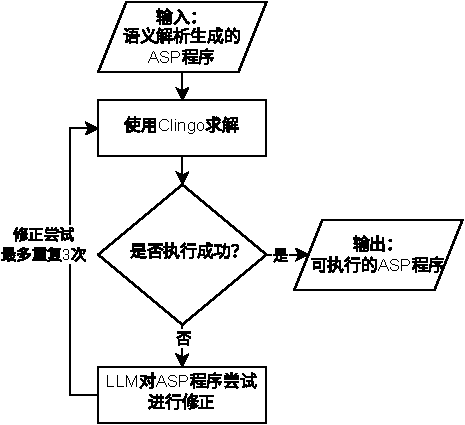
\includegraphics{figures/rule-fix-crop.pdf}
\caption{规则修正流程图}
\label{figure:rule-fix}
\end{figure}
\begin{enumerate}[nosep]
\item 使用Clingo求解器对语义解析模块生成的ASP程序尝试执行。
\item 如果执行成功,没有提示错误,则无需进行进一步修正,直接将ASP程序流转到框架的下一模块。
\item 如果执行失败,则将错误的ASP程序和Clingo求解器提示的错误信息,一起输入LLM,由LLM尝试进行修正。
\item 将修正后的ASP程序再次输入到Clingo求解器中,尝试执行。如此循环最多3次,最终输出经过优化后的ASP程序,流转到框架的下一模块。
\end{enumerate}
\subsubsection{任务定义}
本模块的任务建模为:给定错误的ASP程序和Clingo错误信息,生成一个修正后的ASP程序。采用DSPy的Signature结构表示如下:
\begin{lstlisting}
class FixASPProgram(Signature):
    error_code = dspy.InputField(desc="Clingo返回的错误的ASP代码")
    error_type = dspy.InputField(desc="Clingo报错的类型")
    error_message = dspy.InputField(desc="Clingo报错的提示信息")
    corrected_code = dspy.OutputField(desc="修正后的ASP程序")
\end{lstlisting}
\subsubsection{提示词设计}
针对常见的ASP程序错误类型,本文设计了多组提示模板,包括以下几类:
\begin{table}[H]
\centering
\caption{常见ASP程序错误类型与修正策略}
\begin{tabular}{|l|p{5.5cm}|p{5.5cm}|}
\hline
\textbf{错误类型} & \textbf{描述} & \textbf{修正策略} \\
\hline
语法错误 & 缺少句点、括号不匹配、非法符号等 & 补齐缺失符号或调整语法结构 \\
\hline
基础化错误 & 不安全变量未绑定 & 增加正文字面量以绑定变量 \\
\hline
逻辑错误 & 冲突规则或条件导致无解 & 注释掉冲突规则或添加前提条件 \\
\hline
谓词未定义 & 使用未声明的谓词或拼写错误 & 添加定义或修正谓词名称 \\
\hline
负循环依赖 & 循环依赖中含有否定项 & 拆解规则结构,引入新谓词或添加约束 \\
\hline
\end{tabular}
\end{table}
每类错误对应一个标准化任务描述、错误信息段、以及格式规范的修复输出示例。如下为语法错误的提示示例,其它类型的提示词在附录\ref{appendix:rule-fix}中展示,此处不再赘述。
\begin{lstlisting}
任务描述:请根据提供的 ASP 程序和 Clingo 错误信息,对程序进行修正。

错误类型:语法错误(Syntax Error)—— 缺少句点。

Clingo错误信息:
<stdin>:3:1: error: syntax error, unexpected IDENTIFIER, expecting '.' or ':
  node(b)

错误程序:
node(a).
node(b)  % <- 缺少句号
edge(a,b).

修正后程序:
node(a).
node(b).
edge(a,b).
\end{lstlisting}
使用DSPy的\texttt{Example}对这一类few-shot结构进行封装,结构如下所示,以供后续提示词优化中的优化器使用。
\begin{lstlisting}
from dspy import example

examples = [
    Example(
        inputs={
            "error_code": "node(a). node(b) edge(a,b). path(X,Y) :- edge(X,Y). path(X,Z) :- edge(X,Y), path(Y,Z).",
            "error_description": "Missing period at the end of rule.",
            "error_type": "<stdin>:3:1: error: syntax error, unexpected IDENTIFIER, expecting '.' or ':node(b)"
        },
        outputs={
            "corrected_code": "node(a). node(b) edge(a,b). path(X,Y) :- edge(X,Y). path(X,Z) :- edge(X,Y), path(Y,Z)."
        }
    ),
    ...
]
\end{lstlisting}
\subsubsection{提示词优化}
在构建示例后,使用DSPy的 FewShotPromptOptimizer 对提示词结构进行自动优化:
\begin{lstlisting}
from dspy.optimize import FewShotPromptOptimizer

optimizer = FewShotPromptOptimizer(devset=validation_set, metric=syntax_semantic_match_score)
optimized_module = optimizer(FixASPProgram)
\end{lstlisting}
此处选择FewShotPromptOptimizer的理由与“语义解析”模块中选择FewShotPromptOptimizer的理由类似,
该优化器会对 few-shot 示例进行排序、筛选与重组合,并根据验证集的“语法/语义正确率”反馈来自动调整提示组合,从而获得最优提示配置。

此处的评价指标与“语义解析”模块中同样,选择语法正确率与语义正确率,自定义评价函数\texttt{syntax\_semantic\_match\_score}的定义
自然同样与“语义解析”模块中的自定义评价函数类似,此处不再赘述。

这种方式相比手工设计提示更为稳定、系统性强,且不依赖参数更新,能更好适应不同LLM(如GPT-4、LLaMA3等) 。

\subsection{规则蒸馏}
规则蒸馏的流程如图\ref{distill-process}所示,分为RCNSP运行前构建ASP知识库的规则蒸馏,以及处理VQA请求时补充ASP知识库的规则蒸馏。
本节将依次对这两种情形的规则蒸馏进行介绍,并介绍蒸馏过程中的性能优化方法。
\begin{figure}[h]
    \centering
    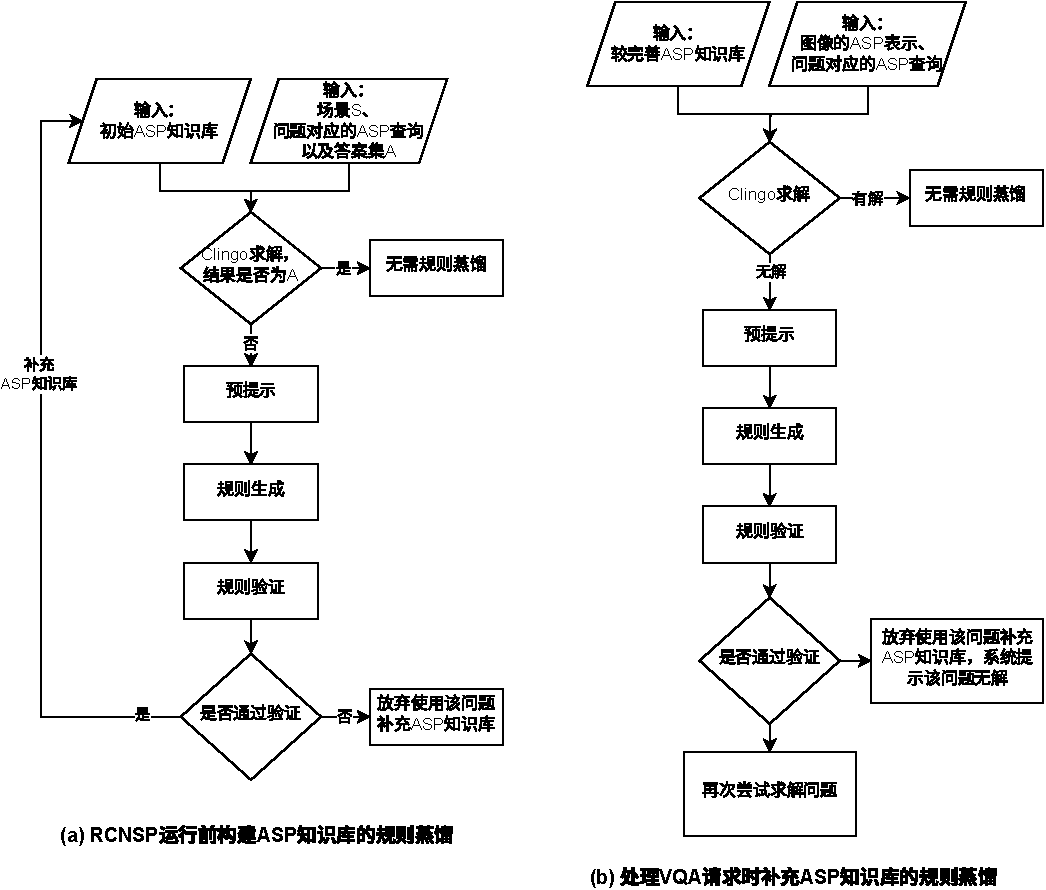
\includegraphics[scale=0.9]{figures/distillation.drawio-crop.pdf}
    \caption{规则蒸馏流程图}
    \label{distill-process}
\end{figure}
\subsubsection{RCNSP运行前构建ASP知识库的规则蒸馏}
RCNSP运行前构建ASP知识库的规则蒸馏的目的是:在RCNSP运行前,利用本文构建的积木世界VQA数据集POVQAD中的问题与答案,引导LLM
自动生成用于解决部分可见积木世界场景下的空间推理VQA问题的ASP规则,并补充到ASP知识库中,以供后续RCNSP运行时解决用户问题时使用。

初始ASP知识库是规则蒸馏的起点,其中包含了一些人工编写的、部分完备的规则集合,用于支持VQA系统在一定程度上进行最基本的逻辑推理。
执行VQA任务的过程中,问题的多样性和复杂性导致很难一次性将解决问题所需的所有知识都填充到ASP知识库中。
因此,需要构建一个初始ASP知识库,后续再不断在解决问题的过程中总结、归纳经验,对其拓展和完善。

初始ASP知识库的构建遵循“最小可运行”的原则,即在保证系统能够正确回答部分问题实例的前提下,
仅包含最基本的一些ASP规则。这样做一方面保证了系统可以运行并进行基本验证,另一方面也为LLM提供了清晰、结构化的理论框架,
使其可以基于已有规则进行合理补全。

初始ASP知识库中通常包含以下几个方面的规则:
\begin{enumerate}[nosep]
\item 基本推理操作规则,包括属性过滤(如\texttt{filter\_color}、\texttt{filter\_shape})、
对象选择(\texttt{select})、合取与析取(\texttt{and}、\texttt{or})、数量计算(\texttt{count})、
布尔值判断(\texttt{exist}、\texttt{verify\_attr}、\texttt{verify\_rel})等等。例如:
\begin{lstlisting}
state(TO,ID) :- scene(TO), object(ID).  % 初始状态:每个object都在scene中
state(TO,ID) :- select(TO, TI, CLASS), state(TI, ID), has_attr(ID, class, CLASS).
bool(TO,yes) :- or(TO, TI0, TI1), bool(TI0,yes).
ans(V) :- end(TO), attr(TO,V).
:- not ans(_).  % 强制必须产生答案
\end{lstlisting}
以上这些规则都使用变量表达,而非常量,以保持泛化能力。
\item 根据数据集中常见问题需求构建规则。POVQAD中,问题均围绕物体的属性、物体的区域位置进行提问。
可以根据数据集中的问题类型,构建一些常见的规则,例如针对提问目标物体的颜色的问题,可能要用到物体的
其它属性、所在的区域等信息来间接推理,可以构建\texttt{filter\_shape}、\texttt{fiter\_region}、
\texttt{filter\_material}、\texttt{filter\_size}规则,
其作用是根据物体的形状、区域、材质、大小等属性进行过滤,从而帮助找出目标物体。
\end{enumerate}

在初始ASP知识库构建完成后,使用本文构建的POVQAD中的训练集来引导LLM进行规则蒸馏,利用LLM自身知识生成扩展规则以补充初始ASP知识库。
对POVQAD训练集中所有样例的场景、问题的ASP表示、问题对应的答案集抽取出来,形成数据集$D$,作为引导LLM进行规则蒸馏的数据源。
随后,对数据集$D$中的第$i$条样例,将其场景$S_i$、问题的ASP表示$QA_i$,与ASP知识库中的所有ASP规则,一同输入Clingo进行求解,
获得答案集$A^*_i$。

如果Clingo求解获得的答案集$A^*_i$与数据集$D$中的答案集$A_i$完全相同,则说明ASP知识库中已经涵盖了足以解决该问题的所有规则,
此时无需再使用LLM进行规则蒸馏。若求解过程中报错或者$A^*_i$与$A_i$并不完全相同,则可认为当前ASP知识库中并不包含解决该问题
所需的全部规则,需要进行规则蒸馏。

规则蒸馏算法的核心包括以下三个环节:预提示、规则生成、规则验证。
预提示在LLM生成新规则之前进行,作用是为LLM提供背景信息和任务说明。具体而言,预提示包括以下内容:

新生成的规则在通过语法检查和规则一致性检查后,将被追加至初始ASP知识库中,
以支持对更广泛问题的解答。语法检查通过Clingo对新生成规则试运行来实现,若没有错误,则认为语法正确;
规则一致性检查通过将新生成规则与现有规则进行合并,
然后用Clingo进行求解,若没有出现错误,表明没有出现ASP规则互相矛盾的情况,则认为规则一致性检查通过。

通过这种基于“最小起点+增量学习”的构建思路,实现了初始ASP知识库向任务完备理论的动态演进,
兼顾了系统可解释性、扩展性与开发效率。

ASP知识库的自动拓展包括以下几个步骤:预提示、规则生成、规则验证,下面按顺序依次进行介绍。

预提示的作用是,为LLM开展后续的规则生成提供背景信息和任务说明,是一组提示词的集合,其包括以下几个方面:
\begin{enumerate}[nosep]
\item \textbf{任务介绍}:简要说明 VQA 任务的背景,告诉 LLM 任务的性质————给定一个问题、
一个图像和它们的描述,生成相应的答案。
\item \textbf{语言语法}:介绍 ASP 规则的基本语法和约定。具体而言,ASP 使用了一些类似于逻辑
程序设计的语法,如:-(表示规则的条件)和 not(表示否定)。
\item \textbf{场景与问题解释}:解释如何将图像场景和问题转换成 ASP 的表示方式。
\item \textbf{答案格式}:告诉LLM如何表示和返回问题的答案。
\item \textbf{初始ASP知识库}:提供初始的ASP知识库$K$,能够回答部分问题,但可能做不到回答所有问题。
\item \textbf{任务说明}:解释LLM在预提示之后将接收的输入以及用户预期的响应。
\end{enumerate}
以上各部分提示词的详细设计方案在附录\ref{appendix:preprompt}中均有介绍。

在向LLM进行预提示之后,进入规则生成环节。此时,将问题的ASP表示、场景一同作为附加提示,要求LLM生成新的ASP规则。
生成的规则是尽可能一般化的规则,即包含更多的变量和较少的常量,以便可以适用于
更广泛的情况。在生成时,可以向LLM直接指明要求其生成尽可能一般化的规则。
一种例如,如果问题是“这只杯子是什么颜色?”,LLM可能会生成以下ASP规则:
\begin{lstlisting}
color_of_cup(Color) :- object(Cup), has_attr(Cup, color, Color), class(Cup,cup).
\end{lstlisting}
这条规则表示:“如果某个物体是杯子,并且它有颜色属性,那么可以推理出它的颜色”。

规则生成之后,需要验证生成的规则是否正确。这一过程需要进行语法
检查、语义检查和回归测试。

语法检查的目的是:检查生成的规则是否符合 ASP 的语法要求。如果规则存在语法错误,
例如拼写错误或格式不对,ASP 解析器将无法解析这些规则。在这种情况下,系统会将错误
信息反馈给 LLM,并要求 LLM 进行迭代反馈修正。

语义检查的目的是:检查生成的规则是否能够配合原有规则,获得预期的答案。如果
不能通过语义检查,则采取“反馈+重试”的方法试图进行修正:将Clingo输出的答案与期望的标准答案一同作为追加提示
提供给LLM,并且新的提示词中会明确告知LLM“你之前生成的规则未能得到正确答案,请你根据下面的输入修改规则。”,
LLM会基于原问题、场景、当前规则结果与目标答案的对比,尝试修复逻辑错误或补全缺失的中间推理步骤。
对同一个示例最多允许修正尝试的次数设为m,其默认值为1,表示失败一次就修正一次,防止过多LLM调用。
若修正后仍失败,说明当前LLM无法处理该示例,跳过或保留当前状态。

语法检查和语义检查都是涉及LLM对ASP程序进行修正,故采用规则修正中经过训练的LLM来完成此处的
语法检查和语义检查任务。

回归测试的目的是:在扩展 ASP 理论的同时,确保新规则不会导致旧问题的答案错误。这
一设计主要基于以下几方面的考量:
\begin{enumerate}[nosep]
\item \textbf{维护系统稳定性和一致性}: 在软件工程中,回归测试被广泛应用于验证新代码的引入
是否影响现有功能的正确性。类似地,在 VQA 系统中,每当通过知识蒸馏添加新规则
时,需要确保这些规则不会干扰系统对先前问题的解答。
\item \textbf{应对模型更新带来的潜在风险}: 知识蒸馏的过程涉及从教师模型向学生模型传递知识,
可能导致学生模型的行为发生变化。通过回归测试,可以检测并防止新知识引入后对模
型性能的负面影响。
\item \textbf{借鉴软件开发中的最佳实践}: 在软件开发中,回归测试是确保新功能或修改不会引入
新错误的关键步骤。将这一理念应用于 VQA 系统,有助于在不断扩展和优化系统的同
时,保持其可靠性和准确性。
\end{enumerate}

回归测试的具体步骤如下:基于更新后的 ASP 理论,重新执行所有历史测试用例,确保
所有旧问题仍然能得到正确答案。如果某个旧问题的答案被破坏,则回退到先前的 ASP 理论,并要求 LLM 重新修正生成的规则。
通过上述设计,回归测试在ASP知识库自动拓展过程中起到了关键的质量保证作用,确
保系统在不断学习和扩展的同时,保持其稳定性和可靠性。

语法检查、语义检查和回归测试这三个环节中,任意一处的修正经多次尝试失败后,系统将视为该问题暂时无法解决,会进行跳过处理,不将该问题用于补充ASP知识库。
\subsubsection{处理VQA请求时补充ASP知识库的规则蒸馏}
处理VQA请求时补充ASP知识库的规则蒸馏的目的是:当RCNSP的ASP知识库中的知识不足以解决用户提出的积木世界VQA问题时,
基于图像场景的ASP表示、问题的ASP表示,引导LLM自动生成能够解决该问题的ASP规则,并补充到ASP知识库中,以供求解该问题及后续类似问题
使用。

ASP知识库经过自动拓展之后,包含了一定量的知识,能够处理一些POVQAD中的一些问题。
用户将自然语言问题和对应积木世界图像输入RCNSP,经过语义解析、视觉场景理解、规则修正后,
由规则蒸馏模块进行处理。与框架初始化阶段进行ASP知识库构建时的规则蒸馏不同,运行时规则自动拓展的目的是:
利用ASP知识库中已有的知识,对用户输入的问题、图像所对应的ASP规则进行补充,以解决部分可见积木世界场景中的
空间推理问题。

判断是否需要进行规则自动拓展的依据是:将问题的ASP表示$QA_i$与场景的ASP表示$S_i$共同输入Clingo,查看是否能够得到答案。若出现语法错误或者无解,则表明
当前ASP规则不足,需要进一步补充。若能够输出与问题相关的ASP谓词(如,问题提问的是不可见物体的颜色,输出谓词也是与颜色相关),则表明
已经有足够的解决问题的规则,不需要进一步补充,直接将$QA_i$和$S_i$继续向后传递到ASP求解器中进行正式求解即可。

此处拓展规则的设计思路与ASP知识库自动拓展中的思路基本相同,不同的点在于,此处输入的只有问题的ASP表示$QA_i$、
场景的ASP表示$S_i$,而不包括问题的答案。由于输入LLM的提示发生了变化,因而提示词也有所变化。
最终接收的输出是新生成的ASP规则。在生成过程中,同样也进行规则验证,并采用反馈重试的方法试图进行修正。
\subsubsection{蒸馏性能优化}
POVQAD训练集中包含数万个样例,如果直接对样本进行蒸馏,既耗时又可能引入冗余信息。
因此,为了提高蒸馏效率,本文提出了样例选择策略,以减少无关数据的干扰。具体而言,包
括以下两种方法:
\begin{enumerate}[nosep]
\item \textbf{谓词计数策略}:该策略根据 ASP 问题表示中谓词的数量对实例进行分组。 分组方法是:
统计每个问题表示中出现的谓词数量,并将具有相同谓词数量的问题归为一组。 通过
这种分组方式,可以根据问题的复杂度(即涉及的谓词数量)来选择示例。 这有助于
LLM 在训练过程中逐步学习,从处理简单问题(谓词数量少)开始,逐步过渡到复杂问
题(谓词数量多),从而提高生成规则的准确性和泛化能力。
\item \textbf{谓词相关性策略}:该策略根据 ASP 问题表示中涉及的具体谓词对实例进行分组。分组
方法是: 识别每个问题表示中出现的谓词,并将包含相同谓词的问题归为一组。 通过
这种分组方式,可以确保 LLM 针对特定谓词学习相关规则。 这有助于 LLM 深入理解
每个谓词的作用和使用场景,从而生成更精确的 ASP 规则,提升 VQA 系统在处理涉及
特定谓词的问题时的表现。
\end{enumerate}

谓词计数策略的设计借鉴了课程学习的思想。课程学习是一种训
练策略,强调按照从易到难的顺序逐步引入训练样本,以提高模型的学习效果。谓词计数策
略通过问题复杂度的分层,体现了课程学习的理念,使模型能够在逐步增加的复杂度中稳定
学习。

在自然语言处理和知识表示领域,基于谓词的特征选择方法被广泛应用于文本分类和信
息检索等任务。谓词相关性策略吸取了这一方法的经验,通过关注问题中涉及的具体谓词,利
用领域知识进行特征选择,确保模型关注于最相关的信息,提高推理的准确性。

为了进一步提高效率,本文还提出了批量优化策略,即一次性给 LLM 多个示例,而不是
逐个示例地生成规则。这一策略借鉴自 Ge\cite{ge2021selfdistillationbatchknowledgeensembling} 等人提出的批量知识集成的自蒸馏方法。 在知
识蒸馏领域,批量知识集成方法通过在同一小批量内传播和整合样本间的知识,生成更精确
的软目标,从而提升模型性能。此外,自蒸馏方法利用模型自身的预测作为训练目标,减少
对外部教师模型的依赖,简化训练流程。

采用批量优化策略,具有以下几点突出优势:
\begin{enumerate}[nosep]
\item \textbf{提高训练效率}: 通过在同一批次内处理多个样本,模型可以并行学习不同样本的特征
和模式,减少训练时间。
\item \textbf{增强模型泛化能力}:批量优化允许模型在一个批次内接触多样化的数据,帮助模型学习
更广泛的特征表示,从而提升对未见数据的适应能力。
\item \textbf{优化资源利用}:通过批量处理,能够更有效地利用计算资源,减少训练过程中的开销。
\end{enumerate}

综合来看,批量优化策略通过借鉴批量知识集成和自蒸馏等方法,旨在提升知识蒸馏过
程中的训练效率和模型性能。
\subsection{ASP推理}
ASP推理阶段中,ASP求解器接收经过优化后的ASP查询语句、视觉场景理解模块提取的ASP事实以及自动拓展的ASP规则,
进行逻辑推理,最终获得答案。
本文使用Clingo求解器来进行求解,其工作过程分为基础化(grounding)阶段和求解(solving)阶段。

基础化阶段将ASP程序中的变量替换为常量,生成一个新的ASP程序。Clingo
通过使用内置的基础化器分析程序,生成所有可能的规则。例如,对规则
$a(X) :- b(X), not c(X).$,其将被展开为所有可能的值为X的实例。

求解阶段中,Clingo采用类似SAT求解器的冲突驱动答案集求解(CDNL)方法。CDNL方法通过迭代地添加约束,
直到找到一个满足所有约束的解,或者证明无解。
具体而言,Clingo基于如下步骤进行求解:(1)初始化。从空分配开始(没有原子被标记为真);
(2)选择与分配。选择一个未分配的原子,猜测其真值为真或假;
(3)传播。根据当前分配和规则,推导其他原子的真值。例如,若规则$a :- b, not c.$满足,b为真且c不在答案集中,则a必须为真;
(4)冲突检测。若分配导致规则冲突(如与已有的约束条件相抵触),记录冲突原因;
(5)回溯与学习。若发生冲突,回溯到之前的选择点,学习冲突子句以避免未来类似错误;
(6)验证。当所有原子分配完成后,检查是否为答案集,即确保它是程序的模型,且最小化(无子集也能满足规则)。

相比其它的ASP求解器,Clingo在以下几个方面进行了优化:(1)从冲突中学习
新的规则,为将来进一步的搜索提供指导;(2)使用多线程实现并行化,同时搜索
多个路径,加速求解过程;(3)使用启发式方法决定分配顺序,例如优先选择高影响力的原子;
(4)预测可能发生的冲突,选择可能导致冲突的原子优先分配,减少搜索空间。
\subsection{求解结果翻译}
经过Clingo得到的输出结果,以形式化的ASP谓词表示,难以直接为最终用户所理解,对用户而言并不友好,需要将其转为自然语言。
Clingo输出的是由逻辑谓词构成的答案集,例如谓词\textbf{left(A,B)}表示“A位于B的左侧”。
由于正常情况下,Clingo输出的都是预先定义的谓词,故采用构造同义词字典的方案,将ASP中的逻辑谓词与自然语言
表述对应起来,作为模板对LLM进行提示。LLM可基于这些模板对解析后的逻辑结果进行填充和修正,生成标准化且易于理解的描述。
本文分析了POVQAD的问题和场景中所用到的谓词,设计了同义词字典,具体见附录\ref{appendix:result-translate}。
\section{实验分析}
本节对4.2节中语义解析、规则修正、规则蒸馏这三个环节分别进行实验,验证各部分的性能。
\subsection{语义解析}
本实验目的包括两方面:(1)评估提示词优化策略在积木世界场景下的语义解析任务中的有效性,比较优化前后对LLM输出ASP程序质量的影响;
(2)验证语义解析模块在不同LLMs上的泛化能力。

实验所用的数据集为POVQAD中的验证集,记为$D$。由于语义解析模块接收的输入为自然语言问题,输出为ASP程序,故只需选用
POVQAD中第$i$条样例的以自然语言形式表示的问题$Q_i$以及其对应的使用ASP表示的问题$QA_i$。

在实验中,本文如下设计了3组提示策略:
\begin{table}[H]
\centering
\caption{常见ASP程序错误类型与修正策略}
\begin{tabular}{|l|p{5.5cm}|p{5.5cm}|}
\hline
\textbf{组别} & \textbf{提示策略} & \textbf{描述} \\
\hline
基线方法 & 零样本提示 & 仅用一句指令提示任务目标,无示例对 \\
\hline
人工少样本方法 & 人工构造少样本示例 & 直接提供设计的所有提示词,由LLMs自主学习 \\
\hline
优化提示词方法 & DSPy FewShotPromptOptimizer优化提示 & 在验证集监督下自动优化Few-shot组合 \\
\hline
\end{tabular}
\end{table}
基线方法中,通过直接向LLMs发送任务指令以及验证集$D$中的自然语言问题,考察LLMs自身固有的根据问题生成ASP程序的能力。
人工少样本方法中,首先向LLMs发送人工设计的所有提示词,并指示LLMs学习如何进行ASP程序生成。随后,再向LLMs发送任务指令以及验证集$D$中的自然语言问题,
考察LLMs自主根据提示词学习的能力。
此外,本文将以上3组提示策略均在DeepSeek-R1 Coder、LLaMA3和ChatGPT分别使用,以验证在不同LLMs上的泛化能力。
3种LLM中,既包含DeepSeek-Coder这类轻量级专用模型,也涵盖ChatGPT-4o这类
通用型先进系统,而LLaMA3性能和效率之间取得了平衡,属于居中水平的模型,选取的都是有代表性的LLM,增强实验说服力和可信度。

考核指标选用语法正确率以及语义正确率,在前文中已经有过定义,此处不再赘述。
实验环境的配置方面,CPU为Intel Core i9 12900K,内存为128GB,显卡为2张Nvidia RTX4090。
另外在实验过程中,对实验重复进行5次,以降低LLM采样过程的随机性带来的影响。

实验结果如表\ref{tab:semantic-result}所示,可以看到在3种LLM上,人工少样本方法相比基线方法在语法正确率和语义正确率上均有很大提升,分别平均提升11.3\%和
11.1\%,证明本文设计的提示词对提升积木世界场景下,能够显著提升LLMs根据自然语言问题生成ASP程序的准确率。
另外,在3种不同的LLM上,优化提示词方法又在人工少样本方法的基础上实现了语法正确率和语义正确率的较大提升,
分别平均提升9.3\%和9.9\%,证明
在积木世界VQA的任务背景下,本文采用的DSPy优化提示词方法能够显著增强LLMs学习提示词的效果。
\begin{table}[h]
    \centering
    \begin{tabular}{lcc}
        \toprule
        \textbf{组别} & \textbf{语法正确率} & \textbf{语义正确率} \\
        \midrule
        \multicolumn{3}{c}{\textbf{DeepSeek-Coder 1.3B}} \\
        基线方法 & 42.4\% & 40.1\%\\
        人工少样本方法 & 52.7\% & 48.4\% \\
        优化提示词方法 & 61.8\% & 57.6\% \\
        \midrule
        \multicolumn{3}{c}{\textbf{LLaMA3 70B}} \\
        基线方法 & 65.7\% & 58.2\% \\
        人工少样本方法 & 78.2\% & 77.1\% \\
        优化提示词方法 & 89.6\% & 86.8\% \\
        \midrule
        \multicolumn{3}{c}{\textbf{ChatGPT-4o}} \\
        直接提问 & 77.5\% & 76.2\% \\
        人工少样本方法 & 88.7\% & 82.4\% \\
        优化提示词方法 & 96.2\% & 93.3\% \\
        \bottomrule
    \end{tabular}
    \caption{语义解析中三种提示策略在不同LLMs上的表现}
    \label{tab:semantic-result}
\end{table}

上述实验结果除了可得出以上的直接结论之外,也说明了以下几点:
\begin{enumerate}[nosep]
\item 自动提示优化优于人工经验构造。手动构造少样本示例往往依赖设计者的直觉和经验,而DSPy中的FewShotPromptOptimizer通过实际性能反馈(如验证集精度、程序可执行性)自动搜索、选择和排列示例,能够系统性地找到更优的组合。
这一显著提升表明提示词设计是一个可学习的搜索问题,而非完全凭经验决策的问题。
\item 提示顺序与上下文协同性影响模型输出质量。LLMs对上下文顺序高度敏感。DSPy通过提示顺序搜索,可能隐式发现了能激发正确结构生成的上下文组合模式。而手动构造示例未必能掌握这一“顺序敏感性”。
不仅是什么示例,更重要的是如何排列示例。
\item 提示优化在结构化输出任务中尤为有效。相较于开放式文本生成任务(如摘要、回答),逻辑程序生成任务(如ASP)对输出的结构、格式要求严格,容错性低。优化后的提示提供了更清晰、更统一的模式,引导模型在“格式敏感”任务中更少出错。
提示优化为结构性任务带来的收益非常显著,尤其是语法和语义正确率的提升。
\end{enumerate}
\subsection{规则修正}
本实验目的包括两方面:(1)评估提示词优化策略在积木世界场景下的规则修正任务中的有效性,比较优化前后对LLM修正ASP程序质量的影响;
(2)验证规则修正模块在不同LLMs上的泛化能力。

实验所用的数据集为人工构造的ASP错误程序集,记为$E$。该数据集的构造目标是:构造一组三元组数据\texttt{(错误的ASP程序,问题文本,修正后的ASP程序)}。
这些样例数据可以作为输入-反馈对,用于提示词优化过程中的\texttt{FewShotPromptOptimizer}。

$E$构造按照如下步骤进行:
\begin{enumerate}[nosep]
\item 从POVQAD中采样一批VQA问题及其标准ASP程序,对POVQAD中第$i$条样例,选取
自然语言表述的问题$Q_i$以及该问题对应的ASP表示形式$QA_i$,组合构成$E$中某条样例数据$e_i$,形式如下:
\begin{lstlisting}
问题: 左边的红色立方体是什么颜色的?
正确程序ₜ:
:- not color(obj1, red).
:- left(obj1, obj2).
:- shape(obj1, cube).
\end{lstlisting}
\item 向正确的ASP程序中人为引入可控错误,获得错误ASP程序$W$。根据前述章节中总结的常见ASP错误类型,此处引入的错误种类包括以下几种:
语法错误、基础化错误、逻辑错误、谓词未定义、负循环依赖。
\item 执行错误程序$W$并筛选语义正确样本。对每个$W$,使用Clingo执行该程序,保留那些程序语法正确但语义错误的样本(即可以执行但输出错误答案的),再排除
语法错误或者无解的极端样本。
\item 构造训练样本对,对某条完整的训练样本,形式如下:
\begin{lstlisting}
指令:以下ASP程序存在错误,请结合问题文本进行修改。
问题:What is the color of the object that is on the left of the red cube?
错误程序:
:- not color(obj1, red).
:- right(obj1, obj2). 
:- shape(obj1, cube).
正确程序:
:- not color(obj1, red).
:- left(obj1, obj2).
:- shape(obj1, cube).
\end{lstlisting}
\end{enumerate}

在实验中,本文如下设计了3组提示策略:
\begin{table}[H]
\centering
\caption{常见ASP程序错误类型与修正策略}
\begin{tabular}{|l|p{5.5cm}|p{5.5cm}|}
\hline
\textbf{组别} & \textbf{提示策略} & \textbf{描述} \\
\hline
基线方法 & 零样本提示 & 仅用一句指令提示任务目标,无示例对 \\
\hline
人工少样本方法 & 人工构造少样本示例 & 直接提供设计的所有提示词,由LLMs自主学习 \\
\hline
优化提示词方法 & DSPy FewShotPromptOptimizer优化提示 & 在验证集监督下自动优化Few-shot组合 \\
\hline
\end{tabular}
\end{table}
基线方法中,通过直接向LLMs发送任务指令以及验证集$D$中的自然语言问题,考察LLMs自身固有的修正ASP程序的能力。
人工少样本方法中,首先向LLMs发送人工设计的所有提示词,并指示LLMs学习如何进行ASP规则修正。随后,再向LLMs发送任务指令以及验证集$E$中的规则修正示例,
考察LLMs自主根据提示词学习的能力。
此外,本文将以上3组提示策略均在DeepSeek-R1 Coder、LLaMA3和ChatGPT分别使用,以验证在不同LLMs上的泛化能力。

考核指标选用三轮以内修复成功率以及修复后语义正确率。
实验环境的配置方面,CPU为Intel Core i9 12900K,内存为128GB,显卡为2张Nvidia RTX4090。
另外在实验过程中,对实验重复进行5次,以降低LLM采样过程的随机性带来的影响。

实验结果如表\ref{tab:rule-fix-result}所示,可以看到人工少样本方法相比基线方法在三轮以内修复成功率和修复后语义正确率上均有很大提升
,分别平均提升11.6\%和7.1\%,证明本文设计的提示词在提升积木世界VQA的任务背景下,能够显著提升LLMs修正ASP规则的成功率。
另外,优化提示词方法又在人工少样本方法的基础上实现了三轮以内修复成功率和修复后语义正确率的较大提升,分别平均提升4.7\%和7.4\%,证明
在积木世界VQA的任务背景下,本文采用的DSPy优化提示词方法能够显著增强LLMs学习提示词的效果。
\begin{table}[h]
    \centering
    \begin{tabular}{lcc}
        \toprule
        \textbf{组别} & \textbf{三轮以内修复成功率} & \textbf{修复后语义正确率}\\
        \midrule
        \multicolumn{3}{c}{\textbf{DeepSeek-Coder 1.3B}} \\
        基线方法 & 56.3\% & 50.3\%\\
        人工少样本方法 & 69.7\% & 62.1\% \\
        优化提示词方法 & 76.6\% & 72.8\% \\
        \midrule
        \multicolumn{3}{c}{\textbf{LLaMA3 70B}} \\
        基线方法 & 58.1\% & 57.9\% \\
        人工少样本方法 & 68.9\% & 60.6\% \\
        优化提示词方法 & 72.2\% & 65.1\% \\
        \midrule
        \multicolumn{3}{c}{\textbf{ChatGPT-4o}} \\
        直接提问 & 71.9\% & 71.5\% \\
        人工少样本方法 & 82.7\% & 79.1\% \\
        优化提示词方法 & 86.6\% & 85.5\% \\
        \bottomrule
    \end{tabular}
    \caption{规则修正中三种提示策略在不同LLMs上的表现}
    \label{tab:rule-fix-result}
\end{table}

\subsection{规则蒸馏}
规则蒸馏实验的目的为:评估本文设计的ASP规则蒸馏方法对提升部分可见积木世界场景下空间推理问答准确率的效果。

为了达到上述实验目的,本节实验对象选取目前主流的三种LLM:DeepSeek-Coder、LLa\-MA3和ChatGPT-4o。
以上既包含DeepSeek-Coder这类轻量级专用模型,
也涵盖ChatGPT-4o这类通用型先进系统,而LLaMA3性能和效率之间取得了平衡,属于居中水平的模型。
在多个基座上进行实验,可以有效证明RCNSP对不同LLM的泛化能力。
实验数据集选取本文第三章构建的POVQAD,将每条样本的图像、自然语言问题输入RCNSP,与每条样本的答案进行对比,计算
回答正确率。实验环境的配置方面,CPU为Intel Core i9 12900K,内存为128GB,显卡为2张Nvidia RTX4090。

模型一采用直接向 VLM 提问的方式,即将自然语言问题与图像一同输入 VLM,并不给予任何的额外提示。
直接提示VLM的方式虽然简单,却是评估模型的关键基准,因为直接提示方法能够反映模型在没有任何
外部推理辅助机制的情况下,自身对空间问题的处理能力。

模型二为原始框架方法,实际上相当于去除规则蒸馏模块的RCNSP。Wang等人设计的原始框架,是对StepGame、SparQA这种纯文本空间推理数据集
中的问题进行推理解答,不包括视觉场景理解,不支持多模态的输入。故去除规则蒸馏模块的RCNSP实际上相当于Wang等人设计的
框架的支持多模态输入的版本,使其能够顺利在第\ref{dataset}章设计的空间推理数据集上进行实验,
进而与本文添加规则蒸馏模块后的RCNSP框架形成对比。

实验结果见表\ref{tab:overall_comparison}。根据实验结果,RCNSP在三种LLM上均取得了较高的正确率,可以证明
RCNSP在不同的LLM上具有泛化能力。RCNSP相比原始框架方法,在DeepSeek-Coder 1.3B、LLaMA3 70B、ChatGPT-4o三种模型上的回答问题
正确率分别高出9.3\%、9.4\%、8.2\%,平均高出8.96\%,足以证明本文设计的规则蒸馏方法对提升部分可见积木世界场景下空间推理问答准确率
具有显著效果。原始框架方法在三种LLM的问答正确率均超过了直接提问方法,证明支持多模态输入后的神经符号VQA框架对部分可见积木世界场景下
的空间推理问答具有有效性。
\begin{table}[h]
    \centering
    \begin{tabular}{lc}
        \toprule
        \textbf{任务类型} & \textbf{正确率} \\
        \midrule
        \multicolumn{2}{c}{\textbf{DeepSeek-Coder 1.3B}} \\
        直接提问 & 59.4\% \\
        原始框架方法 & 72.5\% \\
        RCNSP & 81.8\% \\
        \midrule
        \multicolumn{2}{c}{\textbf{LLaMA3 70B}} \\
        直接提问 & 65.7\% \\
        原始框架方法 & 70.2\% \\
        RCNSP & 79.6\% \\
        \midrule
        \multicolumn{2}{c}{\textbf{ChatGPT-4o}} \\
        直接提问 & 71.5\% \\
        原始框架方法 & 76.6\% \\
        RCNSP & 84.8\% \\
        \bottomrule
    \end{tabular}
    \caption{不同模型及方法在各问题类型上的表现}
    \label{tab:overall_comparison}
\end{table}
\section{本章小结}
本章围绕设计一个规则自动补全的神经符号VQA框架的目标,从设计方案、核心技术及实现与实现分析三方面进行展开。

首先,介绍了RCNSP设计方案。围绕RCNSP的整体设计思路展开,与现有的神经符号框架进行对比,介绍各个模块的功能作用,并重点突出了规则蒸馏中规则自动补充的原理。

其次,介绍了RCNSP核心技术及实现。针对RCNSP中视觉场景理解、语义解析、规则修正、规则蒸馏、ASP推理、求解结果翻译
这六个核心模块进行了详细阐述。特别是对于语义解析、规则修正和规则蒸馏这三个模块进行了重点描述。

最后,进行了实验分析。在第三小节中,本文对语义解析微调实验、规则修正与规则蒸馏实验,从实验目的、实验对象、实验方法、实验环境及实验结果
分析上进行了阐述。
最终语义解析微调实验的结果证明了语义解析模块中,经过微调后的LLM在生成ASP程序方面的语法命中率和语义命中率均有明显提升。
规则修正与规则蒸馏实验的结果证明
神经符号方法对部分可见积木世界场景下空间推理问答有效,本文设计的ASP规则蒸馏方法可以显著提升部分可见积木世界场景下空间推理问答准确率,
同时也验证了RCNSP在不同LLM上具有泛化能力。

本章的RCNSP为后续开发积木世界VQA系统奠定了坚实基础。